\documentclass[tikz]{standalone}
\usepackage{tikz}

\begin{document}

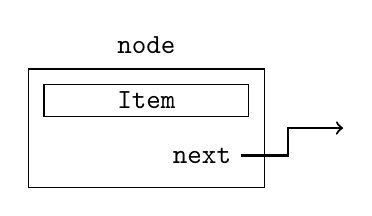
\begin{tikzpicture}[every node/.style={font=\ttfamily}, x=1cm, y=1cm]

% Label above the node
\node at (1.5, 1.8) {node};

% Node 1 (full box)
\draw (0, 0) rectangle (3, 1.5);
\draw (0.2, 0.9) rectangle (2.8, 1.3);
\node at (1.5, 1.1) {Item};
\node[anchor=east] (next1) at (2.7, 0.4) {next};

\draw[->, thick] (next1.east) -- ++(+0.6, 0) |- (4, 0.75);

\end{tikzpicture}

\end{document}